\documentclass[8pt]{article}
\author{
  Saad, MNOUNY
}

    \usepackage[breakable]{tcolorbox}
    \usepackage{parskip} % Stop auto-indenting (to mimic markdown behaviour)
    
    \usepackage{iftex}
    \ifPDFTeX
    	\usepackage[T1]{fontenc}
    	\usepackage{mathpazo}
    \else
    	\usepackage{fontspec}
    \fi

    % Basic figure setup, for now with no caption control since it's done
    % automatically by Pandoc (which extracts ![](path) syntax from Markdown).
    \usepackage{graphicx}
    % Maintain compatibility with old templates. Remove in nbconvert 6.0
    \let\Oldincludegraphics\includegraphics
    % Ensure that by default, figures have no caption (until we provide a
    % proper Figure object with a Caption API and a way to capture that
    % in the conversion process - todo).
    \usepackage{caption}
    %\DeclareCaptionFormat{nocaption}{}
    %\captionsetup{format=nocaption,aboveskip=0pt,belowskip=0pt}

    \usepackage{float}
    \floatplacement{figure}{H} % forces figures to be placed at the correct location
    \usepackage{xcolor} % Allow colors to be defined
    \usepackage{enumerate} % Needed for markdown enumerations to work
    \usepackage{geometry} % Used to adjust the document margins
    \usepackage{amsmath} % Equations
    \usepackage{amssymb} % Equations
    \usepackage{textcomp} % defines textquotesingle
    % Hack from http://tex.stackexchange.com/a/47451/13684:
    \AtBeginDocument{%
        \def\PYZsq{\textquotesingle}% Upright quotes in Pygmentized code
    }
    \usepackage{upquote} % Upright quotes for verbatim code
    \usepackage{eurosym} % defines \euro
    \usepackage[mathletters]{ucs} % Extended unicode (utf-8) support
    \usepackage{fancyvrb} % verbatim replacement that allows latex
    \usepackage{grffile} % extends the file name processing of package graphics 
                         % to support a larger range
    \makeatletter % fix for old versions of grffile with XeLaTeX
    \@ifpackagelater{grffile}{2019/11/01}
    {
      % Do nothing on new versions
    }
    {
      \def\Gread@@xetex#1{%
        \IfFileExists{"\Gin@base".bb}%
        {\Gread@eps{\Gin@base.bb}}%
        {\Gread@@xetex@aux#1}%
      }
    }
    \makeatother
    \usepackage[Export]{adjustbox} % Used to constrain images to a maximum size
    \adjustboxset{max size={0.9\linewidth}{0.9\paperheight}}

    % The hyperref package gives us a pdf with properly built
    % internal navigation ('pdf bookmarks' for the table of contents,
    % internal cross-reference links, web links for URLs, etc.)
    \usepackage{hyperref}
    % The default LaTeX title has an obnoxious amount of whitespace. By default,
    % titling removes some of it. It also provides customization options.
    \usepackage{titling}
    \usepackage{longtable} % longtable support required by pandoc >1.10
    \usepackage{booktabs}  % table support for pandoc > 1.12.2
    \usepackage[inline]{enumitem} % IRkernel/repr support (it uses the enumerate* environment)
    \usepackage[normalem]{ulem} % ulem is needed to support strikethroughs (\sout)
                                % normalem makes italics be italics, not underlines
    \usepackage{mathrsfs}
    \usepackage{caption}

    
    % Colors for the hyperref package
    \definecolor{urlcolor}{rgb}{0,.145,.698}
    \definecolor{linkcolor}{rgb}{.71,0.21,0.01}
    \definecolor{citecolor}{rgb}{.12,.54,.11}

    % ANSI colors
    \definecolor{ansi-black}{HTML}{3E424D}
    \definecolor{ansi-black-intense}{HTML}{282C36}
    \definecolor{ansi-red}{HTML}{E75C58}
    \definecolor{ansi-red-intense}{HTML}{B22B31}
    \definecolor{ansi-green}{HTML}{00A250}
    \definecolor{ansi-green-intense}{HTML}{007427}
    \definecolor{ansi-yellow}{HTML}{DDB62B}
    \definecolor{ansi-yellow-intense}{HTML}{B27D12}
    \definecolor{ansi-blue}{HTML}{208FFB}
    \definecolor{ansi-blue-intense}{HTML}{0065CA}
    \definecolor{ansi-magenta}{HTML}{D160C4}
    \definecolor{ansi-magenta-intense}{HTML}{A03196}
    \definecolor{ansi-cyan}{HTML}{60C6C8}
    \definecolor{ansi-cyan-intense}{HTML}{258F8F}
    \definecolor{ansi-white}{HTML}{C5C1B4}
    \definecolor{ansi-white-intense}{HTML}{A1A6B2}
    \definecolor{ansi-default-inverse-fg}{HTML}{FFFFFF}
    \definecolor{ansi-default-inverse-bg}{HTML}{000000}

    % common color for the border for error outputs.
    \definecolor{outerrorbackground}{HTML}{FFDFDF}

    % commands and environments needed by pandoc snippets
    % extracted from the output of `pandoc -s`
    \providecommand{\tightlist}{%
      \setlength{\itemsep}{0pt}\setlength{\parskip}{0pt}}
    \DefineVerbatimEnvironment{Highlighting}{Verbatim}{commandchars=\\\{\}}
    % Add ',fontsize=\small' for more characters per line
    \newenvironment{Shaded}{}{}
    \newcommand{\KeywordTok}[1]{\textcolor[rgb]{0.00,0.44,0.13}{\textbf{{#1}}}}
    \newcommand{\DataTypeTok}[1]{\textcolor[rgb]{0.56,0.13,0.00}{{#1}}}
    \newcommand{\DecValTok}[1]{\textcolor[rgb]{0.25,0.63,0.44}{{#1}}}
    \newcommand{\BaseNTok}[1]{\textcolor[rgb]{0.25,0.63,0.44}{{#1}}}
    \newcommand{\FloatTok}[1]{\textcolor[rgb]{0.25,0.63,0.44}{{#1}}}
    \newcommand{\CharTok}[1]{\textcolor[rgb]{0.25,0.44,0.63}{{#1}}}
    \newcommand{\StringTok}[1]{\textcolor[rgb]{0.25,0.44,0.63}{{#1}}}
    \newcommand{\CommentTok}[1]{\textcolor[rgb]{0.38,0.63,0.69}{\textit{{#1}}}}
    \newcommand{\OtherTok}[1]{\textcolor[rgb]{0.00,0.44,0.13}{{#1}}}
    \newcommand{\AlertTok}[1]{\textcolor[rgb]{1.00,0.00,0.00}{\textbf{{#1}}}}
    \newcommand{\FunctionTok}[1]{\textcolor[rgb]{0.02,0.16,0.49}{{#1}}}
    \newcommand{\RegionMarkerTok}[1]{{#1}}
    \newcommand{\ErrorTok}[1]{\textcolor[rgb]{1.00,0.00,0.00}{\textbf{{#1}}}}
    \newcommand{\NormalTok}[1]{{#1}}
    
    % Additional commands for more recent versions of Pandoc
    \newcommand{\ConstantTok}[1]{\textcolor[rgb]{0.53,0.00,0.00}{{#1}}}
    \newcommand{\SpecialCharTok}[1]{\textcolor[rgb]{0.25,0.44,0.63}{{#1}}}
    \newcommand{\VerbatimStringTok}[1]{\textcolor[rgb]{0.25,0.44,0.63}{{#1}}}
    \newcommand{\SpecialStringTok}[1]{\textcolor[rgb]{0.73,0.40,0.53}{{#1}}}
    \newcommand{\ImportTok}[1]{{#1}}
    \newcommand{\DocumentationTok}[1]{\textcolor[rgb]{0.73,0.13,0.13}{\textit{{#1}}}}
    \newcommand{\AnnotationTok}[1]{\textcolor[rgb]{0.38,0.63,0.69}{\textbf{\textit{{#1}}}}}
    \newcommand{\CommentVarTok}[1]{\textcolor[rgb]{0.38,0.63,0.69}{\textbf{\textit{{#1}}}}}
    \newcommand{\VariableTok}[1]{\textcolor[rgb]{0.10,0.09,0.49}{{#1}}}
    \newcommand{\ControlFlowTok}[1]{\textcolor[rgb]{0.00,0.44,0.13}{\textbf{{#1}}}}
    \newcommand{\OperatorTok}[1]{\textcolor[rgb]{0.40,0.40,0.40}{{#1}}}
    \newcommand{\BuiltInTok}[1]{{#1}}
    \newcommand{\ExtensionTok}[1]{{#1}}
    \newcommand{\PreprocessorTok}[1]{\textcolor[rgb]{0.74,0.48,0.00}{{#1}}}
    \newcommand{\AttributeTok}[1]{\textcolor[rgb]{0.49,0.56,0.16}{{#1}}}
    \newcommand{\InformationTok}[1]{\textcolor[rgb]{0.38,0.63,0.69}{\textbf{\textit{{#1}}}}}
    \newcommand{\WarningTok}[1]{\textcolor[rgb]{0.38,0.63,0.69}{\textbf{\textit{{#1}}}}}
    
    
    % Define a nice break command that doesn't care if a line doesn't already
    % exist.
    \def\br{\hspace*{\fill} \\* }
    % Math Jax compatibility definitions
    \def\gt{>}
    \def\lt{<}
    \let\Oldtex\TeX
    \let\Oldlatex\LaTeX
    \renewcommand{\TeX}{\textrm{\Oldtex}}
    \renewcommand{\LaTeX}{\textrm{\Oldlatex}}
    % Document parameters
    % Document title
    \title{Le monde NLP}
    
    
    
    
    
% Pygments definitions
\makeatletter
\def\PY@reset{\let\PY@it=\relax \let\PY@bf=\relax%
    \let\PY@ul=\relax \let\PY@tc=\relax%
    \let\PY@bc=\relax \let\PY@ff=\relax}
\def\PY@tok#1{\csname PY@tok@#1\endcsname}
\def\PY@toks#1+{\ifx\relax#1\empty\else%
    \PY@tok{#1}\expandafter\PY@toks\fi}
\def\PY@do#1{\PY@bc{\PY@tc{\PY@ul{%
    \PY@it{\PY@bf{\PY@ff{#1}}}}}}}
\def\PY#1#2{\PY@reset\PY@toks#1+\relax+\PY@do{#2}}

\@namedef{PY@tok@w}{\def\PY@tc##1{\textcolor[rgb]{0.73,0.73,0.73}{##1}}}
\@namedef{PY@tok@c}{\let\PY@it=\textit\def\PY@tc##1{\textcolor[rgb]{0.25,0.50,0.50}{##1}}}
\@namedef{PY@tok@cp}{\def\PY@tc##1{\textcolor[rgb]{0.74,0.48,0.00}{##1}}}
\@namedef{PY@tok@k}{\let\PY@bf=\textbf\def\PY@tc##1{\textcolor[rgb]{0.00,0.50,0.00}{##1}}}
\@namedef{PY@tok@kp}{\def\PY@tc##1{\textcolor[rgb]{0.00,0.50,0.00}{##1}}}
\@namedef{PY@tok@kt}{\def\PY@tc##1{\textcolor[rgb]{0.69,0.00,0.25}{##1}}}
\@namedef{PY@tok@o}{\def\PY@tc##1{\textcolor[rgb]{0.40,0.40,0.40}{##1}}}
\@namedef{PY@tok@ow}{\let\PY@bf=\textbf\def\PY@tc##1{\textcolor[rgb]{0.67,0.13,1.00}{##1}}}
\@namedef{PY@tok@nb}{\def\PY@tc##1{\textcolor[rgb]{0.00,0.50,0.00}{##1}}}
\@namedef{PY@tok@nf}{\def\PY@tc##1{\textcolor[rgb]{0.00,0.00,1.00}{##1}}}
\@namedef{PY@tok@nc}{\let\PY@bf=\textbf\def\PY@tc##1{\textcolor[rgb]{0.00,0.00,1.00}{##1}}}
\@namedef{PY@tok@nn}{\let\PY@bf=\textbf\def\PY@tc##1{\textcolor[rgb]{0.00,0.00,1.00}{##1}}}
\@namedef{PY@tok@ne}{\let\PY@bf=\textbf\def\PY@tc##1{\textcolor[rgb]{0.82,0.25,0.23}{##1}}}
\@namedef{PY@tok@nv}{\def\PY@tc##1{\textcolor[rgb]{0.10,0.09,0.49}{##1}}}
\@namedef{PY@tok@no}{\def\PY@tc##1{\textcolor[rgb]{0.53,0.00,0.00}{##1}}}
\@namedef{PY@tok@nl}{\def\PY@tc##1{\textcolor[rgb]{0.63,0.63,0.00}{##1}}}
\@namedef{PY@tok@ni}{\let\PY@bf=\textbf\def\PY@tc##1{\textcolor[rgb]{0.60,0.60,0.60}{##1}}}
\@namedef{PY@tok@na}{\def\PY@tc##1{\textcolor[rgb]{0.49,0.56,0.16}{##1}}}
\@namedef{PY@tok@nt}{\let\PY@bf=\textbf\def\PY@tc##1{\textcolor[rgb]{0.00,0.50,0.00}{##1}}}
\@namedef{PY@tok@nd}{\def\PY@tc##1{\textcolor[rgb]{0.67,0.13,1.00}{##1}}}
\@namedef{PY@tok@s}{\def\PY@tc##1{\textcolor[rgb]{0.73,0.13,0.13}{##1}}}
\@namedef{PY@tok@sd}{\let\PY@it=\textit\def\PY@tc##1{\textcolor[rgb]{0.73,0.13,0.13}{##1}}}
\@namedef{PY@tok@si}{\let\PY@bf=\textbf\def\PY@tc##1{\textcolor[rgb]{0.73,0.40,0.53}{##1}}}
\@namedef{PY@tok@se}{\let\PY@bf=\textbf\def\PY@tc##1{\textcolor[rgb]{0.73,0.40,0.13}{##1}}}
\@namedef{PY@tok@sr}{\def\PY@tc##1{\textcolor[rgb]{0.73,0.40,0.53}{##1}}}
\@namedef{PY@tok@ss}{\def\PY@tc##1{\textcolor[rgb]{0.10,0.09,0.49}{##1}}}
\@namedef{PY@tok@sx}{\def\PY@tc##1{\textcolor[rgb]{0.00,0.50,0.00}{##1}}}
\@namedef{PY@tok@m}{\def\PY@tc##1{\textcolor[rgb]{0.40,0.40,0.40}{##1}}}
\@namedef{PY@tok@gh}{\let\PY@bf=\textbf\def\PY@tc##1{\textcolor[rgb]{0.00,0.00,0.50}{##1}}}
\@namedef{PY@tok@gu}{\let\PY@bf=\textbf\def\PY@tc##1{\textcolor[rgb]{0.50,0.00,0.50}{##1}}}
\@namedef{PY@tok@gd}{\def\PY@tc##1{\textcolor[rgb]{0.63,0.00,0.00}{##1}}}
\@namedef{PY@tok@gi}{\def\PY@tc##1{\textcolor[rgb]{0.00,0.63,0.00}{##1}}}
\@namedef{PY@tok@gr}{\def\PY@tc##1{\textcolor[rgb]{1.00,0.00,0.00}{##1}}}
\@namedef{PY@tok@ge}{\let\PY@it=\textit}
\@namedef{PY@tok@gs}{\let\PY@bf=\textbf}
\@namedef{PY@tok@gp}{\let\PY@bf=\textbf\def\PY@tc##1{\textcolor[rgb]{0.00,0.00,0.50}{##1}}}
\@namedef{PY@tok@go}{\def\PY@tc##1{\textcolor[rgb]{0.53,0.53,0.53}{##1}}}
\@namedef{PY@tok@gt}{\def\PY@tc##1{\textcolor[rgb]{0.00,0.27,0.87}{##1}}}
\@namedef{PY@tok@err}{\def\PY@bc##1{{\setlength{\fboxsep}{\string -\fboxrule}\fcolorbox[rgb]{1.00,0.00,0.00}{1,1,1}{\strut ##1}}}}
\@namedef{PY@tok@kc}{\let\PY@bf=\textbf\def\PY@tc##1{\textcolor[rgb]{0.00,0.50,0.00}{##1}}}
\@namedef{PY@tok@kd}{\let\PY@bf=\textbf\def\PY@tc##1{\textcolor[rgb]{0.00,0.50,0.00}{##1}}}
\@namedef{PY@tok@kn}{\let\PY@bf=\textbf\def\PY@tc##1{\textcolor[rgb]{0.00,0.50,0.00}{##1}}}
\@namedef{PY@tok@kr}{\let\PY@bf=\textbf\def\PY@tc##1{\textcolor[rgb]{0.00,0.50,0.00}{##1}}}
\@namedef{PY@tok@bp}{\def\PY@tc##1{\textcolor[rgb]{0.00,0.50,0.00}{##1}}}
\@namedef{PY@tok@fm}{\def\PY@tc##1{\textcolor[rgb]{0.00,0.00,1.00}{##1}}}
\@namedef{PY@tok@vc}{\def\PY@tc##1{\textcolor[rgb]{0.10,0.09,0.49}{##1}}}
\@namedef{PY@tok@vg}{\def\PY@tc##1{\textcolor[rgb]{0.10,0.09,0.49}{##1}}}
\@namedef{PY@tok@vi}{\def\PY@tc##1{\textcolor[rgb]{0.10,0.09,0.49}{##1}}}
\@namedef{PY@tok@vm}{\def\PY@tc##1{\textcolor[rgb]{0.10,0.09,0.49}{##1}}}
\@namedef{PY@tok@sa}{\def\PY@tc##1{\textcolor[rgb]{0.73,0.13,0.13}{##1}}}
\@namedef{PY@tok@sb}{\def\PY@tc##1{\textcolor[rgb]{0.73,0.13,0.13}{##1}}}
\@namedef{PY@tok@sc}{\def\PY@tc##1{\textcolor[rgb]{0.73,0.13,0.13}{##1}}}
\@namedef{PY@tok@dl}{\def\PY@tc##1{\textcolor[rgb]{0.73,0.13,0.13}{##1}}}
\@namedef{PY@tok@s2}{\def\PY@tc##1{\textcolor[rgb]{0.73,0.13,0.13}{##1}}}
\@namedef{PY@tok@sh}{\def\PY@tc##1{\textcolor[rgb]{0.73,0.13,0.13}{##1}}}
\@namedef{PY@tok@s1}{\def\PY@tc##1{\textcolor[rgb]{0.73,0.13,0.13}{##1}}}
\@namedef{PY@tok@mb}{\def\PY@tc##1{\textcolor[rgb]{0.40,0.40,0.40}{##1}}}
\@namedef{PY@tok@mf}{\def\PY@tc##1{\textcolor[rgb]{0.40,0.40,0.40}{##1}}}
\@namedef{PY@tok@mh}{\def\PY@tc##1{\textcolor[rgb]{0.40,0.40,0.40}{##1}}}
\@namedef{PY@tok@mi}{\def\PY@tc##1{\textcolor[rgb]{0.40,0.40,0.40}{##1}}}
\@namedef{PY@tok@il}{\def\PY@tc##1{\textcolor[rgb]{0.40,0.40,0.40}{##1}}}
\@namedef{PY@tok@mo}{\def\PY@tc##1{\textcolor[rgb]{0.40,0.40,0.40}{##1}}}
\@namedef{PY@tok@ch}{\let\PY@it=\textit\def\PY@tc##1{\textcolor[rgb]{0.25,0.50,0.50}{##1}}}
\@namedef{PY@tok@cm}{\let\PY@it=\textit\def\PY@tc##1{\textcolor[rgb]{0.25,0.50,0.50}{##1}}}
\@namedef{PY@tok@cpf}{\let\PY@it=\textit\def\PY@tc##1{\textcolor[rgb]{0.25,0.50,0.50}{##1}}}
\@namedef{PY@tok@c1}{\let\PY@it=\textit\def\PY@tc##1{\textcolor[rgb]{0.25,0.50,0.50}{##1}}}
\@namedef{PY@tok@cs}{\let\PY@it=\textit\def\PY@tc##1{\textcolor[rgb]{0.25,0.50,0.50}{##1}}}

\def\PYZbs{\char`\\}
\def\PYZus{\char`\_}
\def\PYZob{\char`\{}
\def\PYZcb{\char`\}}
\def\PYZca{\char`\^}
\def\PYZam{\char`\&}
\def\PYZlt{\char`\<}
\def\PYZgt{\char`\>}
\def\PYZsh{\char`\#}
\def\PYZpc{\char`\%}
\def\PYZdl{\char`\$}
\def\PYZhy{\char`\-}
\def\PYZsq{\char`\'}
\def\PYZdq{\char`\"}
\def\PYZti{\char`\~}
% for compatibility with earlier versions
\def\PYZat{@}
\def\PYZlb{[}
\def\PYZrb{]}
\makeatother


    % For linebreaks inside Verbatim environment from package fancyvrb. 
    \makeatletter
        \newbox\Wrappedcontinuationbox 
        \newbox\Wrappedvisiblespacebox 
        \newcommand*\Wrappedvisiblespace {\textcolor{red}{\textvisiblespace}} 
        \newcommand*\Wrappedcontinuationsymbol {\textcolor{red}{\llap{\tiny$\m@th\hookrightarrow$}}} 
        \newcommand*\Wrappedcontinuationindent {3ex } 
        \newcommand*\Wrappedafterbreak {\kern\Wrappedcontinuationindent\copy\Wrappedcontinuationbox} 
        % Take advantage of the already applied Pygments mark-up to insert 
        % potential linebreaks for TeX processing. 
        %        {, <, #, %, $, ' and ": go to next line. 
        %        _, }, ^, &, >, - and ~: stay at end of broken line. 
        % Use of \textquotesingle for straight quote. 
        \newcommand*\Wrappedbreaksatspecials {% 
            \def\PYGZus{\discretionary{\char`\_}{\Wrappedafterbreak}{\char`\_}}% 
            \def\PYGZob{\discretionary{}{\Wrappedafterbreak\char`\{}{\char`\{}}% 
            \def\PYGZcb{\discretionary{\char`\}}{\Wrappedafterbreak}{\char`\}}}% 
            \def\PYGZca{\discretionary{\char`\^}{\Wrappedafterbreak}{\char`\^}}% 
            \def\PYGZam{\discretionary{\char`\&}{\Wrappedafterbreak}{\char`\&}}% 
            \def\PYGZlt{\discretionary{}{\Wrappedafterbreak\char`\<}{\char`\<}}% 
            \def\PYGZgt{\discretionary{\char`\>}{\Wrappedafterbreak}{\char`\>}}% 
            \def\PYGZsh{\discretionary{}{\Wrappedafterbreak\char`\#}{\char`\#}}% 
            \def\PYGZpc{\discretionary{}{\Wrappedafterbreak\char`\%}{\char`\%}}% 
            \def\PYGZdl{\discretionary{}{\Wrappedafterbreak\char`\$}{\char`\$}}% 
            \def\PYGZhy{\discretionary{\char`\-}{\Wrappedafterbreak}{\char`\-}}% 
            \def\PYGZsq{\discretionary{}{\Wrappedafterbreak\textquotesingle}{\textquotesingle}}% 
            \def\PYGZdq{\discretionary{}{\Wrappedafterbreak\char`\"}{\char`\"}}% 
            \def\PYGZti{\discretionary{\char`\~}{\Wrappedafterbreak}{\char`\~}}% 
        } 
        % Some characters . , ; ? ! / are not pygmentized. 
        % This macro makes them "active" and they will insert potential linebreaks 
        \newcommand*\Wrappedbreaksatpunct {% 
            \lccode`\~`\.\lowercase{\def~}{\discretionary{\hbox{\char`\.}}{\Wrappedafterbreak}{\hbox{\char`\.}}}% 
            \lccode`\~`\,\lowercase{\def~}{\discretionary{\hbox{\char`\,}}{\Wrappedafterbreak}{\hbox{\char`\,}}}% 
            \lccode`\~`\;\lowercase{\def~}{\discretionary{\hbox{\char`\;}}{\Wrappedafterbreak}{\hbox{\char`\;}}}% 
            \lccode`\~`\:\lowercase{\def~}{\discretionary{\hbox{\char`\:}}{\Wrappedafterbreak}{\hbox{\char`\:}}}% 
            \lccode`\~`\?\lowercase{\def~}{\discretionary{\hbox{\char`\?}}{\Wrappedafterbreak}{\hbox{\char`\?}}}% 
            \lccode`\~`\!\lowercase{\def~}{\discretionary{\hbox{\char`\!}}{\Wrappedafterbreak}{\hbox{\char`\!}}}% 
            \lccode`\~`\/\lowercase{\def~}{\discretionary{\hbox{\char`\/}}{\Wrappedafterbreak}{\hbox{\char`\/}}}% 
            \catcode`\.\active
            \catcode`\,\active 
            \catcode`\;\active
            \catcode`\:\active
            \catcode`\?\active
            \catcode`\!\active
            \catcode`\/\active 
            \lccode`\~`\~ 	
        }
    \makeatother

    \let\OriginalVerbatim=\Verbatim
    \makeatletter
    \renewcommand{\Verbatim}[1][1]{%
        %\parskip\z@skip
        \sbox\Wrappedcontinuationbox {\Wrappedcontinuationsymbol}%
        \sbox\Wrappedvisiblespacebox {\FV@SetupFont\Wrappedvisiblespace}%
        \def\FancyVerbFormatLine ##1{\hsize\linewidth
            \vtop{\raggedright\hyphenpenalty\z@\exhyphenpenalty\z@
                \doublehyphendemerits\z@\finalhyphendemerits\z@
                \strut ##1\strut}%
        }%
        % If the linebreak is at a space, the latter will be displayed as visible
        % space at end of first line, and a continuation symbol starts next line.
        % Stretch/shrink are however usually zero for typewriter font.
        \def\FV@Space {%
            \nobreak\hskip\z@ plus\fontdimen3\font minus\fontdimen4\font
            \discretionary{\copy\Wrappedvisiblespacebox}{\Wrappedafterbreak}
            {\kern\fontdimen2\font}%
        }%
        
        % Allow breaks at special characters using \PYG... macros.
        \Wrappedbreaksatspecials
        % Breaks at punctuation characters . , ; ? ! and / need catcode=\active 	
        \OriginalVerbatim[#1,codes*=\Wrappedbreaksatpunct]%
    }
    \makeatother

    % Exact colors from NB
    \definecolor{incolor}{HTML}{303F9F}
    \definecolor{outcolor}{HTML}{D84315}
    \definecolor{cellborder}{HTML}{CFCFCF}
    \definecolor{cellbackground}{HTML}{F7F7F7}
    
    % prompt
    \makeatletter
    \newcommand{\boxspacing}{\kern\kvtcb@left@rule\kern\kvtcb@boxsep}
    \makeatother
    \newcommand{\prompt}[4]{
        {\ttfamily\llap{{\color{#2}[#3]:\hspace{3pt}#4}}\vspace{-\baselineskip}}
    }
    

    
    % Prevent overflowing lines due to hard-to-break entities
    \sloppy 
    % Setup hyperref package
    \hypersetup{
      breaklinks=true,  % so long urls are correctly broken across lines
      colorlinks=true,
      urlcolor=urlcolor,
      linkcolor=linkcolor,
      citecolor=citecolor,
      }
    % Slightly bigger margins than the latex defaults
    
    \geometry{verbose,tmargin=1in,bmargin=1in,lmargin=1in,rmargin=1in}
    
    

\begin{document}
    
    \maketitle
    
    

    
    \hypertarget{objectif}{%
\section{Objectif}\label{objectif}}

    Le traitement de langage naturel plus connu sous le nom NLP pour Natural
Language Processing, est un domaine dans lequel l'intelligence
artificielle essaie de comprend et donner du sens aux contenus
textuelles. L'ojectif de cet article est de s'arrêter sur quelques
notions clés du domaine. Le but est faire comprendre l'intuition
générale de ces modèles tant prisées, qui font tant parler d'eux et dont
le domaine d'application peut être vaste et varié.

    En utilisant le NLP, les développeurs peuvent organiser et structurer
les connaissances pour effectuer des tâches linguistiques telles que :
la synthèse/le résumé automatique de contenus textuels, la traduction
d'une langue vers une autre, l'analyse des sentiments (message positif,
message à caractère sensible, \ldots), la reconnaissance vocale ou
encore la segmentation des sujets.

    Le NLP est un domaine applicatif de l'IA assez complexe parce que
comprendre le langage humain, c'est comprendre non seulement les mots,
mais aussi les concepts sous-jacents et la façon dont, liés entre eux,
des mots assez proches peuvent former des phrases complètement
différentes. Dans ce document nous allons essayer de présenter les
différentes techniques existentes pour le traitement de texte, et de
simplifier les notions complexes utilisées par ces technique. On finira
bien évidemment par présenter le modèle qui a permis d'améliorer
considérablement les avancées sur le domaine. Ce modèle n'est autre que
le fameux BERT introduit par Google en 2018. Une fois la partie
théorique abordée on montrera une petite application de ce modèle et
comment on peut l'appliquer facilement sur un jeu de donnée textuel.

    \hypertarget{contexte-et-motivation}{%
\section{Contexte et motivation}\label{contexte-et-motivation}}

    Dans un des précédents projets nous avons pu aider la communauté Stack
Overflow pour leur fournir un module qui pemet de proposer des tags
grâce à une analyse des mots utilisées dans la question. Pour ce faire
nous avons utilisé des méthodes de modélisation qui peuvent être décrite
comme étant des méthode historiques. Cette méthode consiste briévement à
restructurer le texte de tel sorte à supprimer les mots de la langue qui
n'apporte pas beaucoup de sens dans la phrase. Souvent utilisé comme
lien de coordination, ces termes ne permet que de lier les pensées ou
phrases entre elles. Autre méthode utilsée il s'agit de ramener les
différent à leur racine. En combinant ces méthodes nous pouvons alors
comptabiliser le nombre d'occurence des mots et ainsi essayer de deviner
le contexte générale du texte. On voit d'ores et déjà que cette approche
a l'inconvénient de prendre chaque mot indifféremment du contexte dans
lequel il se trouve. Cela veut dire qu'un mot qui a plusieurs sens
différent serait comptabilisé de la même façon peu importe son contexte.
Aussi plus l'utilisation grammaticale est dense et variée plus l'analyse
devient plus compliquée.

    Il va de soi que cette méthode et approche a permis de faire un grand
pas pour pourvoir analyser et traiter du texte grâce à une intelligence
artificielle, cependant elle manque un peu de bon sens et de mise en
contexte du mot. Il manque la compréhension de la construction de la
phrase et aussi peut souvent mal interprété le sens du texte car
l'analyse exclus le contexte du mot.

    L'approche qu'on souhaite aborder est l'utilisation des nouvelles
méthodes de réseaux de neuronnes, transfert learning vu dans le dernier
projet et ainsi profiter du modèle pré-entrainé par Google qui est
devenu depuis sa publication la base de référence de plusieurs avancées
dans le domaine de NLP. Il serait d'autant dommage de finir la formation
OpenClassroom sans pouvoir tester et appliquer les connaissances
acquises avec ce modèle BERT qui fait tant parler de lui.

    \hypertarget{liens-bibliographique}{%
\subsection{Liens bibliographique}\label{liens-bibliographique}}

   Pour pouvoir mettre au point ce projet et cette analyse on s'est inspiré de plusieurs articles, sites et tutoriels. Je vous liste ci-dessous les différentes références utilisées.

\begin{itemize}
\item Jacob Devlin Ming-Wei Chang Kenton Lee Kristina Toutanova, 2019, BERT: Pre-training of Deep Bidirectional Transformers for Language Understanding https://arxiv.org/pdf/1810.04805.pdf
\item Anna Rogers, Olga Kovaleva, Anna Rumshisky, 2020, A Primer in BERTology: What we know about how BERT works https://arxiv.org/pdf/2002.12327v1.pdf
\item Vaswani et al. Attention is all you need (2017) https://arxiv.org/pdf/1706.03762.pdf
\item Ajay Halthor, Transformer Neural Networks - EXPLAINED!, 2020, https://www.youtube.com/watch?v=TQQlZhbC5ps
\item Ajay Halthor, BERT Neural Network - EXPLAINED!, 2020, https://www.youtube.com/watch?v=xI0HHN5XKDo
\item Chris Manning Richard Socher,  Stanford University School of Engineering, Lecture Collection | Natural Language Processing with Deep Learning (Winter 2017), https://www.youtube.com/playlist?list=PL3FW7Lu3i5Jsnh1rnUwq\_TcylNr7EkRe6
\item Prasad Nageshkar, Multi-label Text Classification with BERT and PyTorch Lightning, 2021, https://curiousily.com/posts/multi-label-text-classification-with-bert-and-pytorch-lightning/
\item Michael PhiMichael Phi, Illustrated Guide to LSTM’s and GRU’s: A step by step explanationIllustrated Guide to LSTM’s and GRU’s: A step by step explanation, 2018, https://towardsdatascience.com/illustrated-guide-to-lstms-and-gru-s-a-step-by-step-explanation-44e9eb85bf21
\item Christopher Olah, Understanding LSTM NetworksUnderstanding LSTM Networks, 2015, http://colah.github.io/posts/2015-08-Understanding-LSTMs/http://colah.github.io/posts/2015-08-Understanding-LSTMs/
\item (Martin et al., 2019) Martin, L., Muller, B., Suárez, P.J.O., Dupont, Y., Romary, L., de La Clergerie, É.V., Seddah, D. and Sagot, B., 2019. Camembert: a tasty french language model. arXiv preprint arXiv:1911.03894.(Martin et al., 2019) Martin, L., Muller, B., Suárez, P.J.O., Dupont, Y., Romary, L., de La Clergerie, É.V., Seddah, D. and Sagot, B., 2019. Camembert: a tasty french language model. arXiv preprint arXiv:1911.03894.
\end{itemize}

    \hypertarget{embeddings}{%
\section{Embeddings}\label{embeddings}}

    Le word embedding est une technique qui permet de modéliser chaque mot
d'un dictionnaire sous la forme d'un vecteur à valeurs numériques
réelles. L'idée est que tous les mots ayant un sens similaire aient des
vecteurs très proche. A l'opposé à la méthode one hot encoding qui
consiste à donner une seule valeur numérique positive dans un vecteur
dont la dimension est égale au nombre de mot du dictionnaire, cette
méthode permet de considérer des espaces vectoriels de dimension bien
inférieure au nombre de mots du dictionnaire et d'éviter ainsi les
problèmes liés au ``fléau de la dimension''.

    Dans l'idéal, nous voulons construire un embedding permettant de
réaliser dans l'espace de représentation vectorielle le genre de
relation suivante : « king -- man + woman = queen », à savoir que la
représentation du mot « king » moins celle du mot « man » plus celle du
mot « woman » permet d'obtenir un vecteur proche de celui de « queen »
(Figure ``Word Embedding''), ou encore Paris - France + Pologne =
Varsovie. L'idée étant de montrer que non seulement les mots proches
thématiquement les uns des autres, le seront également une fois projetés
dans l'espace vectoriel considéré, mais aussi que des relations plus
complexes entre différents concepts sont également captés.

\begin{figure}
\centering
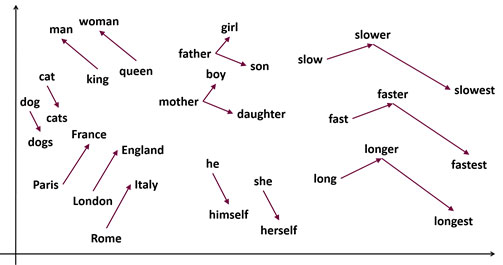
\includegraphics[width=0.5\textwidth]{blog-17-3-1.jpg}
\caption{Word embeddings}
\end{figure}
    

    Généralement de telles représentations sont construites via
l'entraînement d'un réseau de neurones sur des tâches de prédiction.
Concrètement un apprentissage est effectué, sur des corpus gigantesques
de textes via ces réseaux, soit pour prédire un mot en fonction du
contexte (skip-gram), soit pour prédire le contexte en fonction du mot
(bag of words).

    Il est évident que l'intérêt de passer sur une structure vectorielle
permet de faciliter ensuite l'application des méthodes connues de Deep
Learning. Il n'en reste pas moins qu'on peut toujours se poser la
question de quelles combinaison de mots faut il essayer de modéliser
et/ou quelle sous partie du mot.

    \hypertarget{n-grams}{%
\section{N-grams}\label{n-grams}}

    Dans la langue française tout aussi bien que la langue anglaise, on peut
avoir des compositions différentes d'une même racine de mot avec des
suffixes et/ou préfixes. Généralement le préfixe vient à l'opposé de la
racine là ou le suffixe ne change pas beaucoup le sens du mot. Un
embedding pertinent dans ce cas de figure serait de représenter les deux
mots opposés dans deux sens différent là ou les mots similaire dans la
même direction. La considération du N-gram est une technique qui
permettrait de faciliter la modélisation de ces mots.

À titre d'exemple, le bi-gramme le plus fréquent de la langue française
est « de », comme dans l'article « de », mais aussi comme dans les mots
« demain », « monde » ou « moderne ». En traitement du langage naturel
il est plus fréquent de parler de N-gramme pour désigner des séquences
de mots et non de lettres.

C'est le type de modélisation proposée par fastText pour la constitution
de ses embeddings. L'idée est de considérer chaque mot comme l'ensemble
des n-grams qui le constitue, plus le mot lui-même. Par exemple, pour
n=3, le mot « where » est constitué des éléments suivants « \emph{wh »,
« whe », « her », « ere », « re} » et « where ». L'embedding du mot
correspond alors à la somme des tous les vecteurs associés à l'ensemble
des n-grams qui le constituent.

    Regardons un peu comment se déroule les n-grammes appliqué a des
séquences de mots. Prenons les exemples suivants : - San francisco - Les
trois mousquetaires - Il est en retard Bien évidemment il est plus
fréquent de voir San francisco et les trois mousquetaires que la
séquence il est en retard. la dernière séquence de mot est un exemple de
N-grammes pas très fréquent. L'idée est donc d'appliquer de voir la même
succession de mot. Cela permet d'aider à definir quelle combinaison de
mot peut être commme un seul mot, ou encode de faciliter la prédiction
du prochain mot. Autre application peut être aussi de corriger les
erreurs de frappes. Par exemple si on sait que ``café'' à de forte
probabilité d'apparaître après la séquence ``boire du \ldots{}'', on
peut corriger la faute ``caffé'' en faisant une étude de similitude basé
sur les lettres.

    \hypertarget{text-embedding}{%
\section{Text embedding}\label{text-embedding}}

    Traitons le cas du texte embedding. Souvent il est plus pertinent de
considérer plus de mot, notamment pour l'exercice de classification de
texte ou de la génération d'un résumé. Il existe alors plusieurs façons
de procéder : - faire la moyenne de l'embedding associé aux mots de la
phrase ; - effectuer une moyenne pondérée (par exemple avec les poids
calculés via procédure TF-IDF, une mesure statistique caractérisant
l'importance, en nombre d'occurrences, du mot dans un texte ou un corpus
donné).

De telles approches sont possibles mais ne sont pas toujours les mieux
adaptées. En effet, elles reviennent à utiliser a posteriori un
embedding de mots qui a été entraîné dans un contexte différent de celui
pour lequel l'embedding de phrase est recherché. Il devient donc
important de bien choisir son modèle d'embedding selon l'application
qu'on souhaite en faire.

Une fois le concept des embeddings bien assimilé, nous pouvons désormais
nous tourner vers les autres grands concepts utilisés dans le cadre
d'une approche deep learning et voir le cheminement menant de ces
concepts à l'état de l'art actuel du NLP.

    \hypertarget{rnn}{%
\section{RNN}\label{rnn}}

    Un réseau de neurones récurrents (RNN) est un type de réseau de neurones
artificiels qui utilise des données séquentielles ou des données de
séries chronologiques. Ce type d'algorithme d'apprentissage profond est
couramment utilisé pour la résolution de problèmes temporels, tels que
la traduction, la reconnaissance vocale et le sous-titrage d'images. On
peut retrouver cet algorithme dans des applications populaires comme
Siri ou Google Translate.

À l'instar des réseaux de neurones à propagation avant (Feedforward) et
convolutifs (CNN), les réseaux de neurones récurrents utilisent des
données d'entraînement pour apprendre. Ils se distinguent par leur «
mémoire » car ils prennent des informations d'entrées antérieures pour
influencer l'entrée et la sortie actuelles. Alors que les réseaux de
neurones profonds traditionnels supposent que les entrées et les sorties
sont indépendantes les unes des autres, la sortie des réseaux de
neurones récurrents dépend des éléments antérieurs de la séquence. Les
événements futurs sont également utiles pour déterminer la sortie d'une
séquence donnée mais les réseaux de neurones récurrents ne peuvent hélas
pas tenir compte de ces événements dans leurs prédictions.

    Les RNN souffre d'une mémoire très courte. Si une séquence est trop
longue, ils ont du mal à propager l'information apprise plus tôt. Ainsi
si on essaie de traiter un paragraphe pour effectuer des prédictions,
RNN pourrait avoir oublié des informations très importantes lues au
début. Autrement dit, si l'état précédent qui influence la prédiction
actuelle n'est pas dans un passé proche, le modèle RNN peut ne pas être
en mesure de prédire avec précision l'état actuel du système.

Le réseau souffre du problème dit ``Vanishing Gradients''. Les gradients
sont les valeurs qui permettent de mettre à jour les poids d'un réseau
de neuronne. Le problème ``Vanishing Gradients'' est observé quand le
gradient devient trop petit en se propageant dans le temps. Si le
gradient devient trop petit il ne contribue plus trop à l'apprentissage.
Dans l'architecture RNN les neuronnes qui reçoivent un petit gradient
arrête d'apprendre, ainsi ils peuvent aussi oublier ce qui a été vu dans
des longues séquences et pour cela avoir une mémoire très courte. Pour y
remédier, la typologie des LSTM est spécifique avec des « cellules »
dans les couches cachées du réseau de neurones.

    \hypertarget{lstm}{%
\section{LSTM}\label{lstm}}

    Le principe du LSTM (Long Short Term Memory) est de garder la trace de
l'influence entre les différents éléments d'une séquence au contraire
des architectures neuronales classiques. Dans le contexte d'une analyse
de texte, il apparaît naturel de déterminer le sens d'un mot à partir de
ceux qui le précèdent (ou qui le suivent). En pratique, la prise en
compte de telles dépendances sur le long terme n'est pas toujours
effectuée de façon efficace par les RNN (Recurrent Neural Networks)
classiques. C'est la raison pour laquelle le principe des LSTM a été
développé en 1997.

Considérons par exemple la phrase ``J'ai grandi en France\ldots{} Je
parle couramment français''. Si nous voulons détecter le dernier mot de
la phrase (français) le contexte proche indique qu'il s'agit
vraisemblablement d'une langue. Néanmoins pour établir le contexte et
deviner laquelle dont il s'agit il faut remonter plus loin jusqu'au mot
France. Cette dépendance à long terme ne peut généralement pas être
établie par les RNN classiques et nécessite alors l'utilisation des
LSTM.

Le principe classique d'une architecture LSTM est d'être composée d'un
ensemble de ``cellules''. Chacune de ces cellules (variantes mises à
part) est composée de trois portes : 
\begin{itemize}
\item une porte d'entrée (input gate) ;
\item une porte de sortie (output gate) ; 
\item une porte d'oubli (forget gate)
\end{itemize}

La porte d'entrée caractérise à quel point la nouvelle valeur courante
doit modifier le contenu de la cellule ou non. La porte d'oubli
caractérise le niveau d'information de la cellule qui sera ou non
conservé par la suite. La porte de sortie sert à caractériser à quel
point la valeur de la cellule participe à l'activation de la cellule.

\begin{figure}
\centering
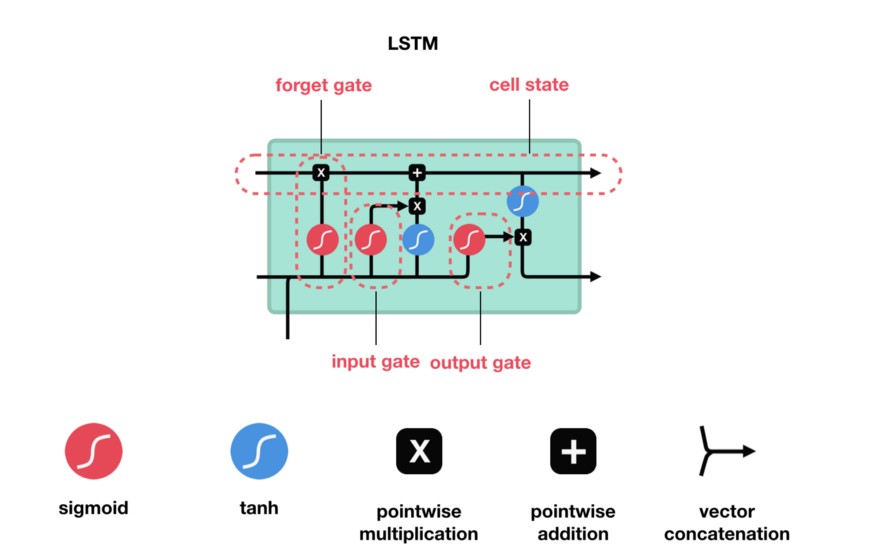
\includegraphics[width=0.5\textwidth]{1_0f8r3Vd-i4ueYND1CUrhMA.png}
\caption{Structure d'un cellule LTSM}
\end{figure}

    Regardons un peu de plus prêt le schéma ci-dessus et essayons de
détailler un peu plus le concept LTSM. Le sigmoid est une fonction
permettant d'avoir une sortie a valeur positive ou nulle. Le tanh est
une fonction permettant de normalisé la sortie pour garder un état avec
des valeurs entre -1 et 1.

Le mécanisme des trois portes va essayer de simuler la fonction de
mémoire de la cellule en n'essayant de garder que des informations
jugées utiles. Dans un premier temps l'information transite par la porte
d'oubli qui peut influencer ou non la remise à 0 de la cellule. La porte
d'entrée quant à elle décide si la nouvelle information doit être
incorporée à l'état de la cellule. Notre nouvel état de cellule est
désormais défini et permettra de déterminer notre sortie. La porte de
sortie va déterminer si l'information reçue doit être incluse dans la
sortie de la cellule.

    Une complexification classique de ce modèle en NLP est le Bidirectional
LSTM dans laquelle on examine à la fois l'information passée mais aussi
l'information future pour analyser une série temporelle. Dans le cadre
de l'analyse d'un texte ou d'une phrase, il apparaît naturel que des
``indices'' concernant la signification d'un mot soient contenus à la
fois sur les mots situés avant mais aussi sur les mots situés après. Une
application typique est l'analyse de sentiment d'une phrase c'est à dire
déterminer si une phrase caractérise un sentiment exprimé plutôt positif
ou plutôt négatif.

Compte tenu de toutes les connexions nécessaires au pilotage de la
cellule mémoire, les couches de neurones de type LSTM sont deux fois
plus ``lourdes'' que les couches récurrentes simples, qui elles-mêmes
sont deux fois plus lourdes que les couches denses classiques.

    \hypertarget{encoder-decoder}{%
\section{Encoder decoder}\label{encoder-decoder}}

    L`Encodeur-Décodeur est un réseau de neurones découvert en 2014 et
utilisé dans de nombreux projet. C'est un pilier fondamental dans les
logiciels de traduction. Le principe d'un encodage est de transformer la
donnée d'entrée en une représentation dans une dimension donnée, puis de
la transformer à nouveau dans un espace plus grand ou plus petit qui
correspond à la dimension de la sortie attendue. Typiquement la
traduction de texte n'est pas quasi littérale, ainsi des mots peuvent
être traduits avec deux mots dans une autre langue, selon le contexte et
plein d'autres paramètres. Regardons de plus prêts cette architecture.

\begin{figure}
\centering
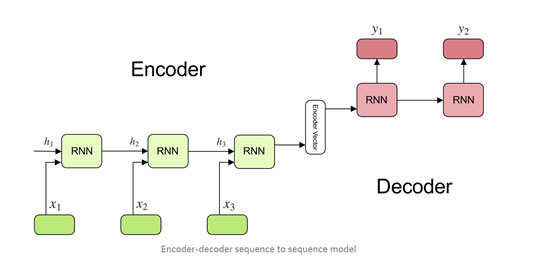
\includegraphics[width=0.5\textwidth]{blog-17-3-5.jpg}
\caption{Architecture Encodeur Décodeur}
\end{figure}

Le modèle se base sur 3 composants : l'encodeur, le vecteur encodé et le
décodeur.

\begin{itemize}
\tightlist
\item
  \textbf{L'encodeur} : Généralement un empilement de plusieurs briques
  RNN (LTSM aussi pour plus de performances) où chacune prend en charge
  un élément de la séquence d'entrée avant de propager l'information
  extraite à la suivante
\item
  \textbf{Le vecteur encodé} : Il correspond à l'état final en sortie de
  l'encoder. La raison d'être de ce vecteur est de contenir
  l'information récupérée via la séquence d'entrée en y rajoutant du
  contexte pour aider le decodeur à en faire en une prédiction
  pertinente. Il sera l'état intial caché du décodeur.
\item
  \textbf{Le décodeur} : Il est constitué d'un empilement de réseaux de
  neurones récurrents (RNN) où chacun prédit un élément de la séquence
  de sortie. Chaque réseau accepte un état caché issu du précédent et en
  envoie un au suivant. La sortie finale est l'ensemble des mots de
  sortie de chaque réseau du decoder.
\end{itemize}

Les Encodeur-Décodeurs sont largement utilisés dans le monde de la
recherche mais ils ont un défaut. Le vecteur que l'Encodeur produit est
fixe. Il va être efficace pour des tâches où la phrase est petite mais
dès que la phrase est trop grande, le vecteur ne va pas pouvoir stocker
toutes l'informations nécessaire. La traduction finale de cette grande
phrase ne sera donc pas très pertinente. Les Encodeur-Décodeurs sont
aujourd'hui couplés à des méchanismes qui leur permettent de s'adapter à
toute longueur de phrase, le mécanisme d'attention.

    \hypertarget{muxe9canisme-dattention}{%
\section{Mécanisme d'attention}\label{muxe9canisme-dattention}}

    L'article ``Attention Is All You Need'' publié par Google Brain et
Google Research en 2017 présentait des techniques pour le calcul
parallèle de masse sur Google TPU. L'attention permet au réseau
d'effectuer un zoom avant précis et de se concentrer sur les mots
contextuels pertinents à la fois dans la séquence d'entrée et dans les
sorties prédites.

L'Attention est une amélioration des Encodeurs-Décodeurs. Au lieu de se
concentrer uniquement sur la sortie finale du RNN, l'Attention va
prélever des informations lors de chacune des étapes du RNN (voir schéma
ci-dessous) :
\begin{figure}
\centering
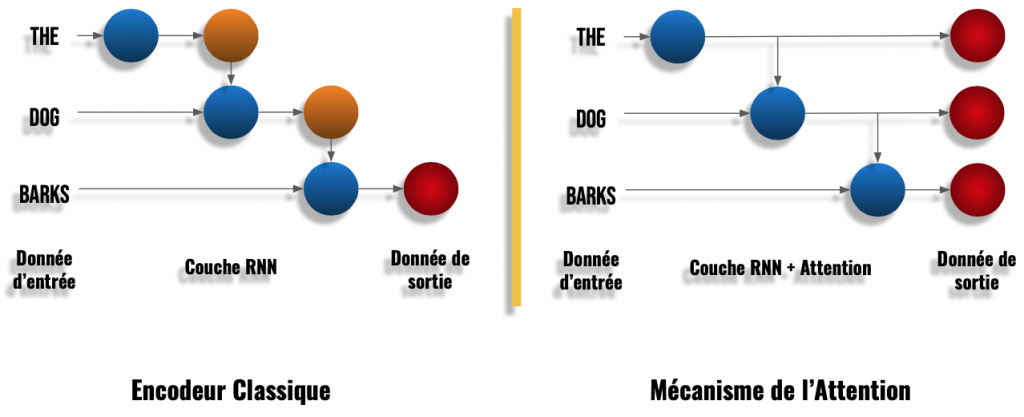
\includegraphics[width=0.5\textwidth]{EncoderVSAttention-1024x417.png}
\caption{Encodeur versus attention}
\end{figure}
On peut voir ci-dessus que dans une couche RNN classique on a une sortie
pour chaque mot. Chaque sortie (ou résultat) sera utilisé pour calculer
la sortie du mot suivant et ainsi de suite. C'est la récurrence. Dans
une couche RNN avec Attention, on a aussi ce calcul récurrent sur chaque
mot. Mais en plus de cela, on garde chacune de ces sorties récurrentes
en mémoire pour former la sortie finale.

Le Décodeur de l'Attention utilise, lui aussi, un RNN mais il ajoute
ensuite d'autres calculs plus complexes.Sa fonction principale est de
comprendre les relations entre chacun des mots. Cette relation va nous
permettre d'identifier les liens qui unissent les mots entre eux. Ainsi
notre modèle va comprendre quel verbe se rapporte à quel sujet, quel
sujet est associé à quel adjectif, etc.

\begin{figure}
\centering
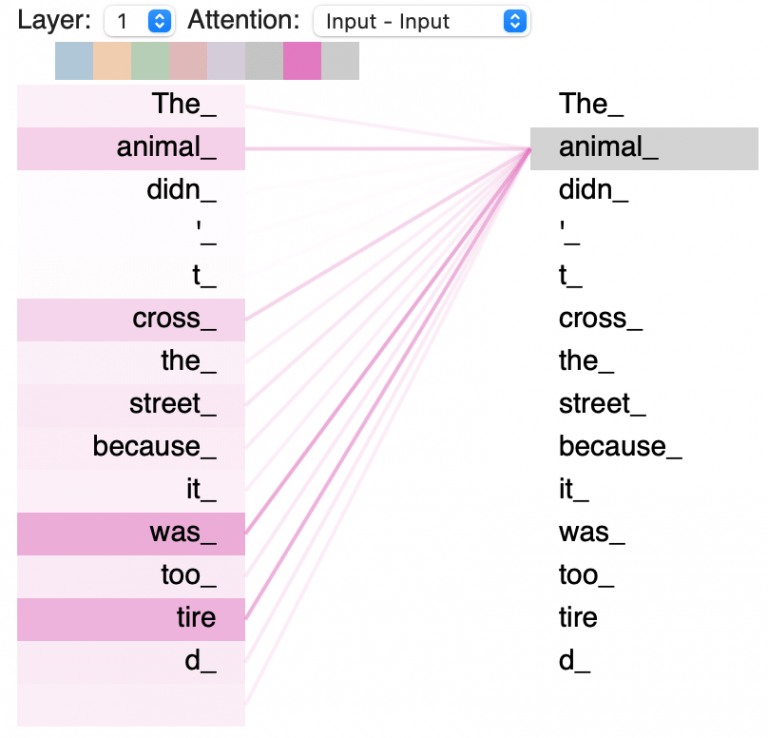
\includegraphics[width=0.5\textwidth]{AttentionViz-768x738.png}
\caption{Lien d'attention}
\end{figure}


Sur ce schéma, on peut voir les liens qui unissent les mots de la phrase
« L'animal n'a pas traversé la rue car il était trop épuisé » (en
anglais) après avoir utilisé le mécanisme de l'Attention. En se
focalisant sur le mot « animal », on peut voir qu'il est directement
relié à « était » et « épuisé ». Ici, l'Attention nous prouve que même
si les mots sont très éloignés dans la phrase, le modèle arrive
comprendre leurs relations. C'est tout l'avantage du mécanisme de
l'Attention. Lors de l'entraînement des réseaux de neurones, le modèle
focalise son attention sur chaque mot de la phrase. Ainsi le modèle peut
détecter le contexte des mots et avoir une compréhension globale de la
phrase.

    \hypertarget{transformers}{%
\section{Transformers}\label{transformers}}

    Le Transformer est un modèle de deep learning qui se caractérise par le
fait qu'il n'a pas besoin de traiter la donnée dans l'ordre, autrement
dit, dans le contexte du NLP, n'a pas besoin de traiter le début d'une
phrase avant sa fin. Cette caractéristique permet au Transformer une
certaine capacité de parallélisation des données (par rapport aux RNN et
CNN). Il est constitué de deux composants principaux à savoir une série
d'encodeurs suivi d'une série de décodeurs. Le principe des LSTM n'est
pas utilisé, ni même celui plus général des réseaux récurrents (RNN).
L'enjeu de garder en mémoire l'information contenue par les mots éloigné
est donc résolu. À chaque instant l'algorithme a accès, sans perte
d'information, à l'ensemble des états successifs parcourus lors de la
procédure. Par contre, il s'appuie fortement sur le principe
d'Attention. En cela, ils constituent une rupture importante d'avec
l'état de l'art précédant leur introduction. L'un des enseignements de
cette approche est que le mécanisme d'attention seul, sans traitement
séquentiel récurrent, est suffisamment puissant pour faire aussi bien,
et mieux, que des RNN avec attention.

\begin{figure}
\centering
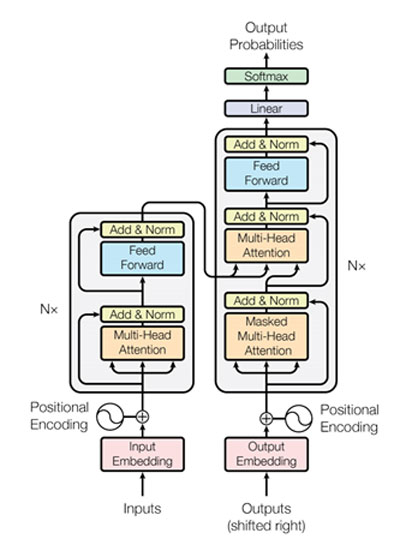
\includegraphics[width=0.5\textwidth]{blog-17-3-7.jpg}
\caption{Architecture de base du Transformer}
\end{figure}

    L'image présente plus précisément l'architecture d'un transformer, le
côté gauche représente l'encodeur là où la partie à droite concerne le
décodeur. Les deux sont composés de plusieurs de plusieurs module
pouvant s'empiler plusieurs fois (Nx dans la figure). Chaque module est
constitué essentiellement de couche ``Multi-Head Attention'' et ``Feed
forward''. Essayons de détailler un peu plus ce modèle de transformer.

Prenons l'exemple d'une traduction d'une phrase d'anglais à français, le
principe est donc d'encoder la phrase en anglais et la décoder par la
suite en français. Comme on le sait très bien les ordinateurs ne
comprennent pas les mots, ils aiment traiter des nombres, des vecteurs
ou des matrices. De ce fait nous appliquons d'abord une représentation
des mots dans un espace d'embedding, ajouté a cela un ``positional
encoding'' qui aide à apporter le bon sens au mot selon le contexte.
Nous avons alors un vecteur avec le bon contexte qui sera traité par la
couche ``Multi-Head Attention''. Cette couche calule plusieurs vecteurs
d'attention pour chaque mot de la séquence. Les vecteurs étant
indépendant nous pouvons alors les paraleliser avant de combiner les
résutltats en appliquant des poids sur les différents vecteurs
d'attention. La couche ``Feed Forward'' permet de transformer les
vecteurs d'attention dans un format compréhensible par le prochain bloc
(Décodeur ou Encodeur).

Notre décodeur prend en entrée de façon séquentielle la sortie de notre
traduction. De la même façon que notre encodeur il transforme notre mot
en français en vecteur et lui ajoute le contexte. Ce vecteur est ensuite
traité par une couche ``Masked Multi-Head Attention'', on parle d'une
couche masqué car il traite l'attention en ayant des mots masqués. Le
résultat notre couche est alors combiné avec le résultat d'attention de
notre décodeur avant de re-rentrer dans une couche qu'on peut appeler
Décodeur-Encodeur d'attention. C'est dans cette couche que la partie
principale de mapping Français Anglais s'effectue. On a en sortie un
vecteur d'attention combiné entre Français et Anglais. Ensuite une
couche feed forward permet de générer un vecteur interprétable soit par
le prochain block de décodeur ou par la couche quui permet de générer
une probabilité de distribution qui est humainement interprétable et qui
à la fin va pouvoir correspondre à un mot avec la plus grande
probabilité.

Ces séquences sont répétées plusieurs fois jusqu'à obtenir la traduction
complète de la phrase et voir le token de fin de phrase. Un Transformer
amélioré spécialisé pour le NLP, BERT, a été introduit quatre ans plus
tard et fait l'objet d'une description ci-dessous.

    \hypertarget{cest-quoi-bert}{%
\section{C'est quoi BERT ?}\label{cest-quoi-bert}}

    BERT est un accronyme anglais : \textbf{Bidirectional Encoder
Representations from Transformers}. Il s'agit d'un modèle créé et publié
par google en 2018. En 2019, Google annone avoir commencé à utiliser ce
modèle dans ses moteurs de recherche. BERT profite de l'architecture des
transfomer en utilisant que la partie gauche du schéma précédent
(L'encodeur), couplé à du traitement bi-directionnelle qui lui permet
d'améliorer sa compréhension des mots et du contexte. Ce modèle
bi-directionnel, est devenu la base de plusieurs recherches dans le
domaine de NLP et a permis des grandes avancées.

    Dans une architecture classique d'un transformer, on a deux parties un
encodeur et décodeur. Dans un exemple de traduction de texte l'encodeur
permet de transformer le texte d'une langue donnée en un vecteur
numérique interprétable par la machine qui contient toute l'information
englobée par la phrase. Le décodeur quant à lui s'occupe de
retransformer ce vecteur numérique dans la langue de traduction. Dans un
sens l'encodeur décodeur peuvent être découplé en deux modules ou deux
tâches ou l'encodeur permet de comprendre la langue et décodeur
d'interpréter la compréhension et la transformer dans un language
humainement interprétable. L'encordeur du tranformer est la base de
l'architecture du BERT qui permet de comprendre une langue. A l'opposé
des autres modèles qui lisait le texte de façon séquentielle, BERT lit
toute la séquence en une fois. Cette caractéristique lui donne le titre
de bi-directionnel là ou en réalité il n'y a pas de direction. Cette
propriété introduite par le principe d'attention permet d'apprendre le
contexte en se basant sur les mots qui sont autour (à gauche ou à
droite).

    Durant son apprentissage BERT utilise deux méthodes : 
\begin{itemize}
\item  MLM : Masked LM.
Avant d'utiliser une séquence de mot BERT masque 15\% des mots de la
séquence, ensuite le modèle essaie de prédire chacun des mots masqués.
Il se base pour cela du context fournit par les mots non masqués. BERT
apprend le lien entre les mots constituants la même phrase
\item  NSP : Next Sentence Prediction. Le modèle reçoit des paires de phrases en entrée et
apprend à prédire si la deuxième phrase est la phrase qui suit dans le
texte originale. Avec cette méthode il essaie de comprendre et prédire
les liens entre les phrases.
\end{itemize}
    Ainsi les applications sont devenues très simple grâce au BERT. Le
modèle pré-entrainé qui a déjà appris la langue peut être utilisé et
fine tuné pour répondre à un besoin très précis en rajoutant une petite
couche au coeur du modèle.

    \hypertarget{comment-utiliser-bert}{%
\section{Comment utiliser BERT ?}\label{comment-utiliser-bert}}

    Dans un document à part nous allons détailler les étapes que nous allons
suivre pour une utilisation du modèle BERT. Pour notre application du
modèle de BERT nous allons utiliser Pytorch Lightening qui est un Deep
Learning framework permettant de faciliter l'implémentation des modèles
Deep Learning.

En terme de données nous reprenons le même jeu de données utilisées dans
le projet de prédiction des tags des questions Stack Overflow. Nous
allons traiter un problème de classification multi label. Autrement dit
une question peut appartenir à plusieurs classes, là où un problème
multi classe veut simplement dire que notre observation ne peut avoir
qu'une seule valeur positve parmi les classes de prédiction.

    Nous n'allons pas trop s'attarder sur l'analayse de notre jeu de donnée
car celle-ci a déjà été effectuée dans le projet précédent. Nous allons
suivre les étapes suivantes : 

\begin{itemize}
\item Charger les données et les prétraiter 
\item Préparer les dataset pytorch et lightening DataModule - Définir le
modèle
\item Entrainer le modèle en utilisant les librairies Lightening Trainer 
\item  Evaluer la performance du modèle

\end{itemize}

    Le modèle BERT a été
pré-entrainé sur plusieurs articles de Wikipédia et de \emph{Book corpus} il a donc
une bonne compréhension de la langue anglaise. Cependant nous souhaitons
l'appliquer sur des questions issues de Stack OverFlow qui sont plutôt
orientés langage de programmation et qui dans bien des cas présente du
code issue d'un langage de programmation. Nous allons voir si BERT
saurait bien s'adapter à ce domaine qui n'est peut être pas le langage
naturel humain.

Pour l'analyse du texte français il existe un modèle pré-entrainé qui a
été utilisé pour apprendre la langue française. Le modèle porte le nom
de \textbf{camenBert}. Un petit jeu de mot pour un petit clin d'oeil à
la communauté française.

    \hypertarget{conclusion}{%
\section{Conclusion}\label{conclusion}}

    Nous avons pu atteindre notre objective de compréhension des différentes
techniques et méthodes utilisées dans le domaine du NLP. Nous avons
montré tous les éléments de modélisation qui précédait l'arrivée du BERT
et qui permet tout aussi de comprendre son fonctionnement. Nous avons
parlé nottamment : 
\begin{itemize}
\item Des méthodes d'embedding, qui permettent de modéliser
des mots en vecteurs
 \item  Des réseaux de neuronnes réccurents qui permet de
se rappeler d'un état antérieur mais souffre d'une petite mémoire 
\item  LTSMs une version améliorée des réseaux de neuronnes réccurent qui
souhaitait corriger le problème de mémoire ou vanishing gradient 
\item Encodeur Décodeur qui permet de réutiliser tous ces composants pour
traiter du texte dans une dimension avant de le décoder dans une autre
dimension 
\item  Le principe d'attention introduit avec les transformer qui
est une version 2.0 des encodeur décodeurs 
\item  Le fameux modèle BERT
introduit par Google qui a réussi comprendre l'anglais et qui avec
lequel plein de nouveaux projets et documents de recherche ont vu le
jour
\end{itemize}

A la fin nous avons montré comment on pouvait mettre en pratique le
modèle BERT en s'attaquant à un problème de classification. Il s'agit
d'un projet traité auparavant que nous avons souhaité abordé
différemment. Dans ce contexte nous avons réussi à améliorer notre
modèle de prédiction de tag des questions Stack Overflow. BERT est donc
facile à utiliser et peut résoudre beaucoup de problèmatique mais
demande comme on l'a vu du temps et des ressources en termes de
puissance de calcul non négigeable.


    % Add a bibliography block to the postdoc
    
    
    
\end{document}
